\chapter{Joint}
    We need to define and characterize what kind of multistable joint we are using. We will do this in this chapter, first covering the basic building block of our joint, and shows how we can compute the position of the joint relative to an input. Secondly we will see how we stacked the basic structure in serie to get multistable joint. 
    
    \section{Bistable joint}
    \label{sec:bistable}
    \begin{figure}
        \centering
        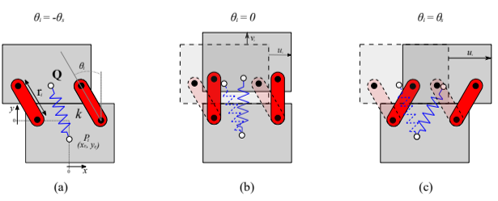
\includegraphics[width=1.0\textwidth]{images/basics_building_blocks.png}
        \caption{Schematics showing our basic building structure. It is composed of one bottom block, considered as fixed, and a top block that we can displace. The two blocks are linked together using arms of length $r_i$ and anchor distance $\delta$ represented in red. A linear spring is also linking the two blocks together, with and anchor on the bottom block that can be changed. This structure is therefore pulling the top block toward the bottom block and depending of the spring anchor location, it will create two stable resting state. If the top block is on the left side, we call this \textit{state 0}, on the right we call this \textit{state 1}}
        \label{fig:joint_basics}
    \end{figure}
    We first start with the basic structure of our joint, which consists of two rectangular blocks, one on top of the other as shown on Figure \ref{fig:joint_basics}. Those two blocks are linked together using 4 arms (2 arms are visible in the 2D view) to constrain the displacement of the top block compare to the bottom one. We consider the bottom block to be connected to the frame, therefore we can have a horizontal input displacement on the top block. The horizontal displacement of the top block is constrained by the length of the arms ($r_i$) and the distance between arm's anchor point to the side of the block ($\delta$). We define $\theta_i$ as the angle between the $y$ (vertical) axis and the longitudinal axis of the arm, it is positive when the block is positioned on the right. $\theta_i$ is constrained between two bounds: $-\theta_s$ and $\theta_s$ that is computed using Equation \ref{eq:theta_s}. Once we know $\theta_s$, we can compute the maximum horizontal travel distance for the top block using Equation \ref{eq:max_dist}. The vertical displacement ($y$) of the block can be computed using $\theta_i$ and Equation \ref{eq:y_block}.
    
    \begin{equation}
        \theta_s = cos^{-1}\left(\frac{2\delta}{r_i}\right)
        \label{eq:theta_s}
    \end{equation}
    \begin{equation}
        bistable\_max\_dist = 2 sin(\theta_s) \cdot r_i
        \label{eq:max_dist}
    \end{equation}
    \begin{equation}
        v_i = cos(\theta_i) \cdot r_i
        \label{eq:y_block}
    \end{equation}
    
    We also have a spring that connects the two block together. This spring has two anchors positions. $Q$ anchor is positioned horizontally in the middle of the top block and vertically at a distance $\delta$ of top block side. $P$ anchor can be positioned arbitrary in the bottom block at the position $(x_P, y_P)$. We will consider the spring as a linear spring with a stiffness $k$ and a rest length $l_0$. The potential energy stored in the spring can be explained using Equation \ref{eq:potential_single} \cite{mo_main_paper}. From Equation \ref{eq:potential_single} we can find a local maximum at Equation \ref{eq:snap_angle} which represent the angle where the block would be at an unstable equilibrium point, meaning if the actuation goes beyond $\theta_{snap}$ from left to right, the top block would snap and rest on the $theta_s$ position. 
    
    From the paragraph above, we observe than the due to the potential energy stored in the spring, the block can have one or two resting states. We will call those : \textit{state 0} when the block is on the left and \textit{state 1} when the block is on the right. This basic structure will help us build a multistable system that will be used to create the legs of our robot.
    

    \begin{equation}
        \epsilon = \frac{k}{2}\left(\sqrt{(r_i sin\theta_i - x_P)^2 + (r_i cos\theta_i - y_P)^2} - l_0^2\right)    
        \label{eq:potential_single}
    \end{equation}
    \begin{equation}
        \theta_{snap} = tan^{-1}\left(\frac{x_P}{y_P}\right)    
        \label{eq:snap_angle}
    \end{equation}
    
    
    
    \section{Multistable joint}\label{sec:mutistable}
        To create a multistable joint, we will use the basic building block as seen in section \ref{sec:bistable} and stack two of them in serie. Figure \ref{fig:joint_multistable} shows how we stack the two bistable joint together. We have three blocks, the bottom block is anchored to the ground, the middle block is linked to the bottom one with two arms of length $r_1$ with and anchor distance of $\delta_1$, we also attached a spring that has a anchor at position $(x_{P_1}, y_{P_1})$. The top block is linked to the middle block in the same way but this time, arms have length $r_2$ and anchor distance $\delta_2$. Also the second block has an anchor point at position $(x_{P_2}, y_{P_2})$. 
        Both bistable joint has their own $theta_{i_1}$, $theta_{i_2}$ and horizontal maximum travel distance.
        
        \begin{figure}
        \centering
        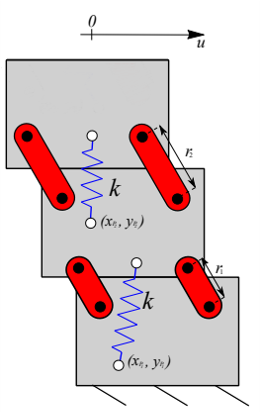
\includegraphics[width=0.40\textwidth]{images/multistable.png}
        \caption{Schematic of a multistable joint build with two bistable joint assembled in serie. Parameters such as arms lengths, springs anchor position define the number of stable states we may have. We can define 4 states: $00$ when $\theta_{i_1} = -\theta_{s_1}$ and $\theta_{i_2} = -\theta_{s_2}$; $01$ when $\theta_{i_1} = -\theta_{s_1}$ and $\theta_{i_2} = +\theta_{s_2}$; $10$ when $\theta_{i_1} = +\theta_{s_1}$ and $\theta_{i_2} = -\theta_{s_2}$; $11$ when $\theta_{i_1} = +\theta_{s_1}$ and $\theta_{i_2} = +\theta_{s_2}$}
        \label{fig:joint_multistable}
        \end{figure}
        
        When stacking multiple blocks together, the total potential energy stored in the stack is described with Equation \ref{eq:potential}  \cite{mo_main_paper}. In this equation, $theta_i$ represent the angle formed by the $i$-th pair of levers with the vertical axis, $r_i$ represent the length of the $i$-th arms, $x_{P_i}$ and $y_{P_i}$ represent the position of the $i$-th spring. As described in M. Zanaty's paper \cite{mo_main_paper}, we can find different configuration of stable position for our three block structure where the potential energy is at a local minimum. Those different position leads use to once again define states. 
        \begin{equation}
            \epsilon_{tot} = \frac{k}{2} \sum_{i=1}^{N}\left(\sqrt{(r_i sin \theta_i - x_{P_i})^2 + (r_i cos \theta_i - y_{P_i})^2} \right) - l_0^2
            \label{eq:potential}
        \end{equation}
        Those states are defined with the same strategy than for bistable block. Each bistable block can be in either \textit{state 1} or \textit{state 2}. As we have two bistable blocks, we will use two numbers to represent the state of the multistable joint. The first number will represent the state of the bottom bistable joint, the second number will represent the state of the top bistable joint. Therefore we have 4 possibles states described below: \\
        \begin{itemize}
            \item $00$ when $\theta_{i_1} = -\theta_{s_1}$ and $\theta_{i_2} = -\theta_{s_2}$; (Both blocks on the left)
            \item $01$ when $\theta_{i_1} = -\theta_{s_1}$ and $\theta_{i_2} = +\theta_{s_2}$; (Middle block on the right, Top block on the left)
            \item $10$ when $\theta_{i_1} = +\theta_{s_1}$ and $\theta_{i_2} = -\theta_{s_2}$; (Middle block on the left, Top block on the right)
            \item $11$ when $\theta_{i_1} = +\theta_{s_1}$ and $\theta_{i_2} = +\theta_{s_2}$; (Both blocks on the right)
        \end{itemize}
        
        Those states will lead to different type of sequences as we will see in Section \ref{sec:sequences}. The multistable structure is actuated from the top block. We define the origin by the \textit{state 00} resting point. We can easily imagine adding more bistable structure above our multistable joint in order to create even more states and possibilities, but for our experiments and analysis, we will stay focused on the 3 blocks tall multistable joint, the analysis for 4 blocks tall is being done in Dr. M. Zanaty's paper \cite{mo_main_paper}.
        
    \subsection{Sequences}\label{sec:sequences}
        Multistable joints have different possible states (\textit{00; 01; 10; 11}), those states may be activated when a specific scenario is triggered. The Equation \ref{eq:potential} shows the potential energy stored in the system for a combination of angles. Depending of the placement of the springs we will have different sequences. A sequence is a particular order of state. We will consider that all our sequences starts from \textit{state 00} and will hit the \textit{state 11} before coming back to the first \textit{state 00}. We can represent those sequences as in a final state machine of 4 states.We can see in Figure \ref{fig:sequences} the different sequences that our multistable will be able to run. 
        
        \begin{figure}
            \centering
            \includegraphics[width=0.8\textwidth]{images/sequennces.png}
            \caption{Schematics showing sequences}
            \label{fig:sequences}
        \end{figure}
        \todo{Need much more explanation and graph}
        
        
    